\documentclass{beamer}

\mode<presentation> {
	\usetheme{Berlin}
}

\title[Annual University Scientific Conference 2018, Veliko Tarnovo, Bulgaria]{
	Mobile Alternative of the MoneyBee Project for Financial Forecasting
}

\author{Petar Tomov, Iliyan Zankinski, Maria Barova}

\date{14-15.VI.2018}

\institute[IICT-BAS, AUSC'18] {
	Institute of Information and Communication Technologies \\ 
	Bulgarian Academy of Sciences \\
	\medskip
	\textit{p.tomov@iit.bas.bg}
}

\begin{document}

\begin{frame}
\titlepage
\end{frame}

\begin{frame}
\frametitle{Overview}
\tableofcontents
\end{frame}

\section{Introduction}

\subsection{Time Series Forecasting}

\begin{frame}
\frametitle{Time Series}
\begin{itemize}
  \item Data points indexed in time order.
  \item Most commonly a sequence taken at successive equally spaced points in time. 
  \item It is a sequence of discrete-time data. 
  \item Time series analysis comprises methods for analyzing time series data in order to extract meaningful statistics.
  \item Time series forecasting is the use of a model to predict future values based on previously observed values.
\end{itemize}
\end{frame}

\subsection{Artificial Neural Networks}

\begin{frame}
\frametitle{Artificial Neural Networks}
\begin{itemize}
  \item Weighted directed graphs.
  \begin{itemize}
    \item Nodes with activation function.
    \item Edges with strength of the connection.
  \end{itemize}
  \item Usually organized in layers.
  \item Training is optimization of the weights which minimize the total error of the output.
  \item Build functional relation between input and output training examples. 
\end{itemize}
\end{frame}

\subsection{Mobile Distributed Computing}

\begin{frame}
\frametitle{MoneyBee Project}
\begin{figure}[h]
  \centering
  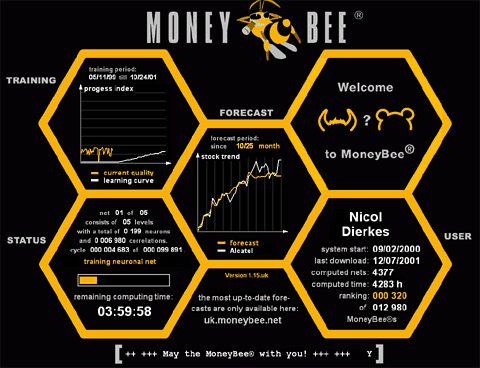
\includegraphics[width=0.75\linewidth]{fig05}
\label{fig:05}
\end{figure}
\end{frame}

\begin{frame}
\frametitle{Donate Distributed Computing}
\begin{itemize}
  \item Kind of parallel computing.
  \begin{itemize}
    \item Problem is divided into many tasks.
    \item Each task is solved by one or more computers.
    \item Computers communicate with each other by message passing.
  \end{itemize}
  \item Usually heterogeneous system.
  \begin{itemize}
    \item Concurrency of components.
    \item Lack of a global clock (synchronization).
    \item Independent failure of components.
  \end{itemize}
  \item Distributed computing is donated when users participate in the system without monetary reward and absolutely volunteer.
  \item When mobile devices are used it is mobile distributed computing.
\end{itemize}
\end{frame}

\section{Technical Solution}

\subsection{Mobile Computing}

\begin{frame}
\frametitle{Android Live Wallpaper}
\begin{itemize}
  \item During most of the operating time, the mobile devices are in idle mode.
  \item Live Wallpaper is interactive background on the Android home screen.
  \item On regular intervals, wallpaper service is activated.
  \begin{itemize}
    \item Cycle of ANN training is executed.
    \item Single forecast is retrieved.
    \item Visual information is updated.
  \end{itemize}
\end{itemize}
\end{frame}

\subsection{Encog Machine Learning Framework}

\begin{frame}
\frametitle{Artificial Neural Network as Java Model}
\begin{itemize}
  \item Multilayer perceptron with 3 layers.
  \item Time series is conditionally divided in two parts (past and future).
  \begin{itemize}
    \item Data frame for the past (lag) is supplied at the input of the ANN.
    \item Time series data are scaled (according neurons activation function) before fed into ANN's input.
    \item Data frame for the the future (lead) is expected at the output of the ANN.
    \item The output is also scaled with the opposite scaling coefficient used at the input.
  \end{itemize}
  \item At each training cycle resilient backpropagation training is executed.
\end{itemize}
\end{frame}

\subsection{Technologies Stack}

\begin{frame}
\frametitle{Software Architecture}
\begin{figure}[h]
  \centering
  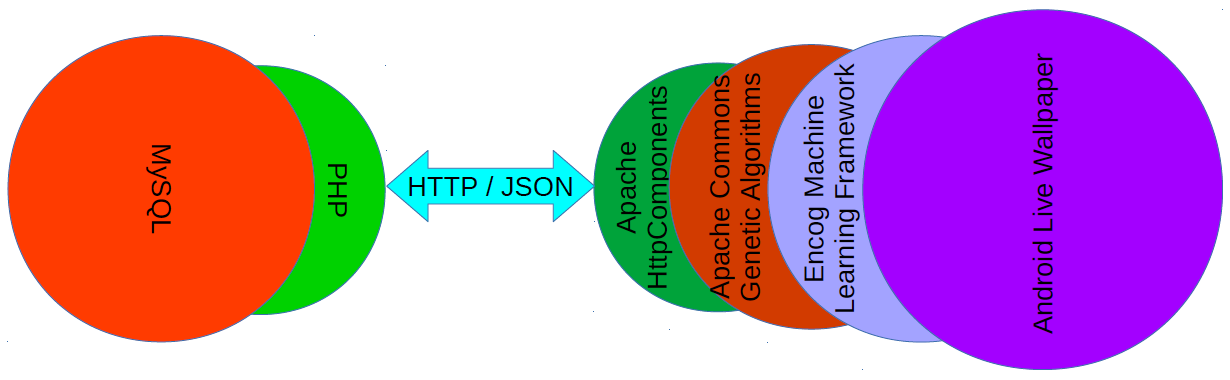
\includegraphics[width=0.75\linewidth]{fig01}
\label{fig:01}
\end{figure}
\end{frame}

\section{Experiments and Results}

\subsection{Wallpaper Settings}

\begin{frame}
\frametitle{Settings Dialog}
\begin{figure}[h]
  \centering
  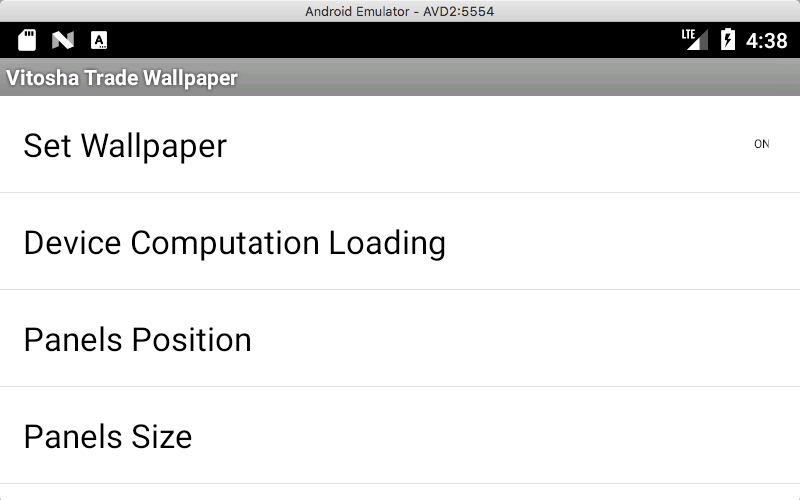
\includegraphics[width=0.75\linewidth]{fig03}
\label{fig:03}
\end{figure}
\end{frame}

\subsection{Wallpaper Setup}

\begin{frame}
\frametitle{Setting the Wallpaper}
\begin{figure}[h]
  \centering
  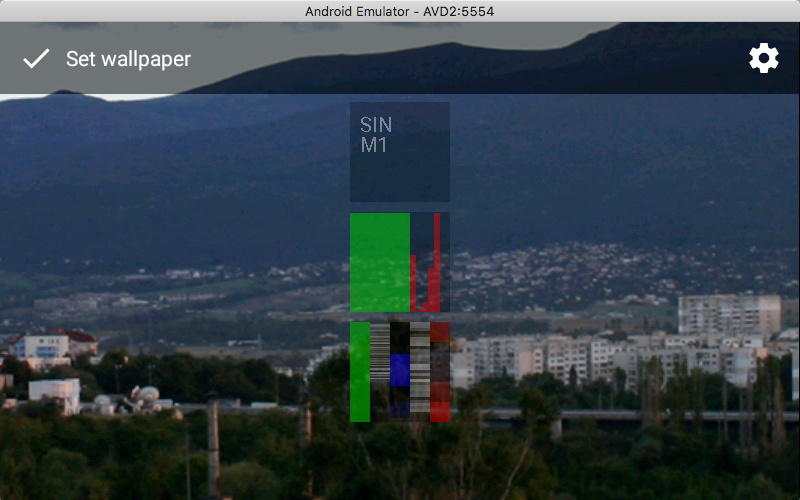
\includegraphics[width=0.75\linewidth]{fig04}
\label{fig:04}
\end{figure}
\end{frame}

\subsection{Wallpaper Running Mode}

\begin{frame}
\frametitle{Background Training and Forecasting}
\begin{figure}[h]
  \centering
  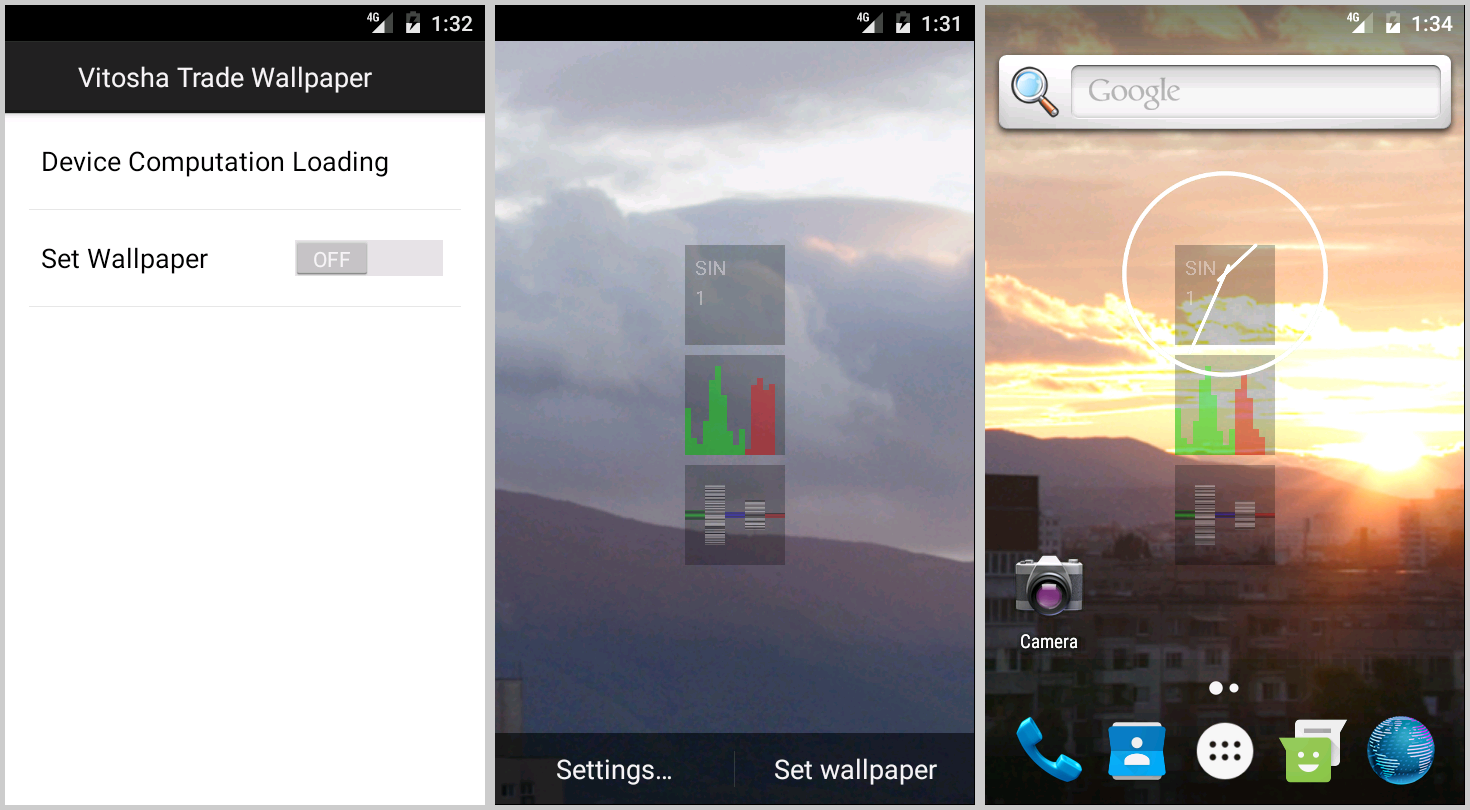
\includegraphics[width=0.75\linewidth]{fig02}
\label{fig:02}
\end{figure}
\end{frame}

\section{Conclusions}

\subsection{Advantages and Disadvantages}

\begin{frame}
\frametitle{Conclusions}
\begin{itemize}
  \item Donated mobile devices power appears to be much more promising even compared to the donated desktop distributed computing.
  \begin{itemize}
    \item Mobile devices are almost always running, which is not the case with the desktop computers.
    \item Mobile devices are less powerful than desktop computers.
  \end{itemize}
\end{itemize}
\end{frame}

\subsection{Q\&A}

\begin{frame}
\frametitle{Questions and Answers}
\center \huge{Thank you for the attention!}
\end{frame}

\end{document}
